\documentclass[b5paper,10pt,twoside]{article}
\usepackage[english]{babel}
\usepackage{graphicx}
\usepackage[utf8]{inputenc}
\usepackage[T1]{fontenc}
\usepackage{times}
\usepackage{amsfonts}
\usepackage{amssymb}
\usepackage{amsthm}
\usepackage[b5paper,centering]{geometry}
\usepackage{fancyhdr}

\usepackage{mathtools}
\usepackage{amsmath}


\setlength\textheight{184mm}
\setlength\textwidth{127mm}

\pagestyle{fancy}
\renewcommand{\leftmark}{P. Janus, T. Kryjak, M. Gorgoń}
\renewcommand{\rightmark}{Tutaj tytuł}
\fancyhead{}
\fancyhead[RE]{\leftmark}
\fancyhead[LE]{\thepage}
\fancyhead[LO]{\rightmark}
\fancyhead[RO]{\thepage}
\fancyfoot{}
\renewcommand{\headrulewidth}{0.4pt}
\renewcommand{\footrulewidth}{0pt}

%\usepackage{titlesec}
\usepackage{enumerate}
% \usepackage{rotating}
%\usepackage[font=small,labelfont=bf,labelsep=period]{caption}
\usepackage{listings}
\usepackage{todonotes}

\lstloadlanguages{Python}  % to nie ma dla nas znaczenia

\lstset{language=Python,
basicstyle=\ttfamily\small,
commentstyle=\ttfamily\small,
classoffset=0,
keywordstyle=\ttfamily\small,
classoffset=1,
keywordstyle=\ttfamily\small,
classoffset=0,
stringstyle=\ttfamily\small,
commentstyle=\ttfamily\itshape\small,
numbers=none,
numberstyle=\ttfamily\small,
identifierstyle=\ttfamily\small,
showstringspaces=false,
morekeywords={
}}

\sloppy
\flushbottom
\setlength{\parindent}{7mm}

%\titlelabel{\thetitle.}
%
%\titleformat{\section}{\bfseries\large}{\filright \thesection . }{0ex}{}
%odstępy: lewy, góra, dół
%\titlespacing{\section}{7mm}{24pt plus 0pt minus 1pt}{12pt plus 0pt minus 1pt}

%\titleformat{\subsection}
%{\bfseries}{\filright \thesubsection.\hspace{7.5mm} }{0ex}{}
%odstępy: lewy, góra, dół
%\titlespacing{\section}{7mm}{24pt plus 0pt minus 1pt}{12pt plus 0pt minus 1pt}

\renewcommand*{\thefootnote}{\fnsymbol{footnote}}


%\renewcommand{\figurename}{\bf Fig.}
%\renewcommand{\refname}{REFERENCES}




\begin{document}
\thispagestyle{empty}

\hrule

\vspace{2mm}

\noindent
AUTOMATYKA/AUTOMATICS $\bullet$ 2019 $\bullet$ Vol. ? $\bullet$ No. ?

\vspace{2mm}

\hrule

\vspace{22mm}

Piotr Janus\footnote{AGH University of Science and Technology, Faculty of Electrical Engineering, Automatics, Computer Science and Biomedical Engineering, Krakow, Poland. e-mail: \{piojanus, tomasz.kryjak, mago\}@agh.edu.pl}, Tomasz Kryjak$^*$, Marek Gorgoń$^*$

\vspace{9mm}


{\bf\Large Tutaj tytuł\\[2mm] \indent cd}

\vspace{12mm}

\noindent
{\small \textbf{Abstract}: Abstract
\vspace{12pt}

\noindent
{\small \textbf{Keywords}: }


\section{Introduction}
\label{sec:introduction}

Foreground object segmentation is one of the most important element of modern AVSS (\textit{Advanced Video Surveillance Systems}. It can be used in a variety of vision systems such as detection and tracking object or human behaviour analysis. Moreover it is a key element of application like abandoned luggage detection or forbidden zone protection. It might be applied in border control and airport systems as well.

%ten akapit ok
%Segmentacja obiektów pierwszoplanowych jest jednym z kluczowych elementów wielu advanced video surveillance systems (AVSS). Jest używana w systemach detekcji i trackowania obiektów oraz human behaviour analysis. Oprócz tego jest również ważnym elementem takich aplikacji jak abadnoned luggage detection and forbidded zone protection. Systemy mogę być użyte w border control i airports).

The simplest group of foreground object detection algorithms
is based on subtracting subsequent frames from a video
sequence. More advanced approaches involve the so-called
background modelling. For each pixel, a dedicated model is
assigned that describes the background appearance in a given
location. Then, depending on used algorithm, the new pixel
value is compared to the background model and classified
(as foreground, background and sometimes also shadow). The
model is updated to incorporate changes in the scene like slow
or fast light variations and movement of objects belonging to
background (i.e a moved chair).

However, BGS approach has some serious limitations such as low adaptation to lighting changes, another weak point is the case when the color of background and foreground object are similar and the objects merge. This phenomenon is called color camouflage and in such a case is hard to retrieve foreground object properly. The main reason is that aforementioned techniques utilized human perception in some ways. Possibly image can be described in another color space (i.e. HSV or YCbCr) but it is still represented as a visible light, which is how people see it. Segmentation accuracy can be improved by using so called depth sensor. It extends the conventional image with depth map which provides the distance between particular pixel and sensor. This device is based on infrared projector and IR camera, projector shoots an irregular pattern of dots, which is invisible to humans, then IR camera is able to detect the infrared light bounced off from our subjects. The same technology is used by Kinect -- Microsoft gaming console. 

%\textbf{TODO} - dlaczego RGB--D jest lepsze, jeden akapit
%TODO TK raczej co daje informacja o D.
%Takie algorytmy mają jednak pewne podstawowe ograniczenia takie jak słaba odporność na zmiany oświetlenia. Drugi słaby punkt to sytuacja gdy kolory tła i przedmiotów pierwszoplanowych są podobne i zlewają się ze sobą. W takiej sytuacji ciężko o prawidłową segmentację obiektów. Spowodowane to jest faktem, że przetwarzany obraz jest takim jak widzi go człowiek, ewentualnie może być przedstawiony w innej przestrzenii barw (np. HSV lub YCbCr). 

%Do analizy można wykorzystać róznież tzw. mapę głębi obrazu. Rozszerza on standardowt obraz o informację o odległości danego piskela od kamery. Tego typu urządzenie działa na zasadzie czujnika na podczerwień, taką technologię wykorzystuje też konsola do gier \textit{Microsoft Kinect}. 


%However, these BGS techniques have some fundamental
%limitations because they utilized human perception (i.e.,
%visible light) based color spaces such as the red, green, and
%blue (RGB), the hue, saturation, and value (HSV) and the
%YUV where Y and UV represent luminance and chrominance,
%respectively. Basically, those methods are weak to
%color camouflage situations and also sensitive to illumination
%changes.


In this paper extended versions of the most commonly used background segmentation algorithms have been proposed. Described methods have been adjusted to image acquired from conventional RGB camera and depth sensor. The main contributions of this paper are:
\begin{itemize}
\item Extended version of Gaussian Mixture Model (GMM) and Pixel--Based--Adaptive--Segmenter (PBAS) algorithms adjusted to be used with conventional RGB image and depth sensor
\item Embedded implementation of aforementioned algorithms on GPU using CUDA architecture
\item Detailed performance comparison between standard (only RGB image) and RGD--D version
\end{itemize}
For image acquisition the sensor from \textit{Intel Real--Sense} series has been used, while computing platform comes from Nvidia Jetson family. Moreover, the difference of performance between embedded platform and PC equipped with dedicated Nvidia Touring GPU is presented.

% The authors have focused on Gaussian Mixture Model (GMM) and Pixel--Based--Adaptive--Segmenter (PBAS) algorithms. In addition to software model, the embedded implementation, with the use of GPU and CUDA architecture, is presented as well.   The authors also verified how does the RGB--D sensor improve the accuracy of particular algorithm comparing to the original version. 

%TODO opis co zostało zrobione
%W niniejszej pracy zaprezentowano rozszerzone wersje powszechnie wykorzystywanych algorytmów do segmentacji obiektów pierwszoplanowych. Opisane metody zostały dostosowane do przetwarzania danych otrzymanych ze standardowej kamery RGB oraz czujnika RGB-D. Skupiono się na algorytmach Gaussian Mixture Model (GMM) i Pixel-Based-Adaptive-Segmenter (PBAS), oprócz modelu programowego przygotowano także implementację wbudowaną w układzie GPU z wykorzystaniem architektury CUDA. 
%%TODO TK nie wiem czy GPU można nazwywać sprzętową... raczej wbudowaną. \cite do metod.
%Do akwizycji obrazu użyto czujnika \textit{Intel Real--Sense} natomiast platforma sprzętowa to \textit{Nvidia Jetson}. Dodatkowo porównano wydajność opisanej platformy z komputerem klasy PC wyposażonym w dedykowaną kartę graficzną. Sprawdzono również jaki rzeczywiście wpływ na dokładność algorytmu ma wykorzystanie składowej głębi.

The reminder of this paper is organized as follows. In section \ref{sec:prev_work} previous work related to use of RGB--D sensor for foreground object segmentation are briefly discussed, a few papers about acceleration using GPU are also presented. Section \ref{sec:algorithms} describes adjusted version of GMM and PBAS method. In section \ref{sec:hw_implementation} the designed embedded system is shown in presented. The evaluation of proposed algorithms is shown in section \ref{sec:evaluation}. The paper ends with a conclusion and future research directions indications.

%Struktura niniejszego artykułu jest następująca, w rozdziale \ref{sec:prev_work} przedstawiono wcześniejsze prace związane z wykorzystaniem czujników RGB--D do segmentacji obiektów pierwszoplanowych. Sekcja \ref{} opisuje sposób przekazywania sygnału pochodzącego z czujnika RGB--D do platformy obliczeniowej oraz architekturę do przetwarzania obrazu w technologi CUDA. Sekcja \ref{} zawiera opis implementacji sprzętowej w układzie Nvidia Jetson. W ostatnim rozdziale zamieszczono podsumowanie oraz wskazano dalsze kierunki rozwoju aplikacji.   

\textbf{TODO:}\\
->wyraźnie zaznaczyć, że to coś nowego i że jest lepsze !!!

\section{Previous work}
\label{sec:prev_work}

%TODO TK Tu musi być jakieś "zagajnie", a nie tak od razu i jeszcze dość niefortunnie (bo inne od czego ?)
Over the years, several solutions for foreground object segmentation with the use of RGB--D sensor have been proposed. Sometimes researcher are also focused on improving performance instead of developing new algorithms. In such a case using GPU is a promising approach. The following section presents previous work related with both RGB--D sensors and GPU implementations.

Authors in \cite{Hoffman_2016} proposed foreground segmentation algorithm which uses  convolutional neural network (CNN). Training data set consists both RGB and depth map images. The main contribution of that paper is improved training process. In order to produce more accurate detection, hybrid system with two CNN working in parallel is proposed. The first one uses conventional RGB image while second network is based on depth map only. The key element of this algorithm is so called mid-level fusion technique between RGB and depth CNNs. According to tests conducted by authors, the use of depth map results in an average 21\% relative improvement in detection performance over an RGB-only network.

%TODO krócej
%Autorzy publikacji \cite{Hoffman_2016} przedstawili inne, bardzo ciekawe i niestandardowe podejście do segmentacji obiektów pierwszoplanowych. 
%Zaprezentowany algorytm zakłada wykorzystanie sieci neuronowa CNN. 
%Do uczenia sieci użyto, oprócz annotowanych danych uczących, także czujnik RGB--D, czyli urządzenie generujące obraz wraz z mapami głębi. 

%Oczywiście istnieje wiele metod segmentacji obiektów pierwszoplanowych, wykorzystujących sieci nieuronowe, w tym przypadku autorzy skupili się na usprawnieniu procesu uczenia. 
%Standardowo w tego typu algorytmach, sieć uczona jest na podstawie annotowanych obrazów w przestrzeni RGB. 
%Zbiory testowe można podzielić na wiele kategorii, jednak uzyskany w ten sposób dokładność detekcji nie zawsze jest zadowalająca. 
%W związku z tym autorzy przedstawili hybrydowy system, w którym równolegle uczone są dwie sieci. 
%Pierwsza z nich wykorzystuje standardowy zbiór obrazów zapisanych w przestrzeni RGB, natomiast w drugiej sieci wykorzystywana jest mapa głębi tego obrazu. W zaproponowanym podejściu kluczową rolę odgrywa wymiana informacji pomiędzy obiema sieciami CNN w trakcie procesu uczenia. 
%Dzięki takiemu rozwiązaniu można dużo efektywniej przeprowadzić taki proces dla obu sieci i następie połączyć je w jedną. 
%TODO TK: Ogólnie opis tego trzeba jakoś inaczej przedstawić, bo to jest niejasne. Tak samo nie wiadomo co za bardzo daje to -D

In the work \cite{Hasnat_2014} another foreground segmentation algorithm which is based on RGB--D sensor was presented. In this case algorithm works without supervision and consists of statistical model based on the color and the geometry of the scene. The authors presented only software model, without embedded or hardware implementation.

Proposed model is used together with a JCSA \textit{Joint Color-Spatial-Axial} clustering method, which is responsible for estimation of background parameters, clustering the pixels and generating the set of regions in the image. The authors proposed hybrid model which uses multivariat Gaussian and Watson distributions. For clustering operation,   
BSC (\textit{Bregman Soft Clustering}) method has been used. The last phase of the algorithm is region merging, for this purpose RAG (ang. \textit{Region Adjacency Graph}) is build. 

Authors compared presented method with another algorithms based on depth image.  Various test for different parameters were conducted, the set of quality indicators was also proposed. The evaluation methodology is based on NYU depth database \cite{}. Test results proved that detection quality is significantly improved comparing to previous solutions.

%W pracy \cite{Hasnat_2014} został zaprezentowany kolejny, bazujący na obrazie z czujnika RGB--D, algorytm segmentacji obiektów pierwszoplanowych. 
%W tym przypadku zaproponowano metodę działającą bez nadzoru, przedstawiony algorytm składa się z mechanizmu grupowania w dziedzinie barw i przestrzeni oraz statystycznego łączenia obszarów. 
%Autorzy niestety nie przedstawili implementacji sprzętowej, przetestowano jedynie model programowy.
%%TODO TK: "sprzętowe" jw. 

%Wykorzystany algorytm grupowania JCSA (ang. \textit{Joint Color-Spatial-Axial clustering}) służy do estymacji parametrów modelu tła, grupowania pikseli i w efekcie wyodrębnienia regionów na obrazie. 
%Sam model tła jest hybrydowy i składa się z rozkładów Gaussa oraz Watsona. 
%Do wspomnianego wcześniej grupowania pikseli użyto algorytmu BSC (\textit{Bregman Soft Clustering}). 
%W ostatniej fazie metody, czyli łączeniu poszczególnych regionów wykorzystano natomiast graf sąsiedztwa (ang. \textit{RAG -- Region Adjacency Graph}), przedstawiony proces polega na łączeniu odpowiednich wierzchołków w grafie.

%Autorzy porównali zaprezentowany algorytm z innymi metodami bazującymi na obrazie głębi. 
%Przeprowadzono testy dla różnych zestawów parametrów i zaproponowano odpowiednie wskaźniki jakości. 
%Wykonane eksperymenty pozwoliły dobrać parametry algorytmu, natomiast uzyskane wyniki potwierdziły wyraźnie większą dokładność w stosunku do zaprezentowanych wcześniej rozwiązań.
%TODO TK: też by się to bardziej precyzyjnie przydało ująć.

%Publikacja \cite{Mattoccia_2015} przedstawia czujnik RGB--D w całości zrealizowany w układzie FPGA. 
%System działa w czasie rzeczywistym z częstotliwością powyżej $30$Hz. 
%Wykorzystano do tego celu układ FPGA Spartan 6, do akwizycji obrazu użyto natomiast czujników Aptina pracujących w rozdzielczości $800x480$ pikseli z częstotliwością $60$Hz. 
%Komunikacja z sensorami odbywa się za pośrednictwem magistrali szeregowej $I^2C$.
%
%W pierwszym kroku przeprowadzana jest operacja rektyfikacji obrazu, otrzymywany sygnał pochodzi z dwóch sensorów konieczne jest zatem znalezienie odpowiadających sobie punktów na obu obrazach. Następnym etapem jest zastosowanie transformaty Censusa i operacja dopasowania stereo. Ostatni krok to złożona filtracja obrazu wyjściowego. Na wyjście systemu przekazywany jest 16 bitowy obraz głębi, który następnie jest przesyłany do hosta za pośrednictwem portu USB. Warto zaznaczyć, że autorzy wykorzystali technikę generacji kodu HLS (ang. \textit{High--Level Synthesis}), dzięki temu większość funkcjonalności została zaimplementowana w języku C i~automatycznie przekonwertowana na VHDL.
%TODO TK: ta publikacja pewnie będzie bez związku z tym konktretym arykułem.


%TODO TK: Tu też zdanie wprowadzenia, bo wczęsniej było RGB-D, a teraz jest GPU.

In the article \cite{Boghdady_2015}, GPU acceleration for Gaussian based foreground segmentation algorithm was proposed. That system is able to handle multiple cameras simultaneously. Unfortunately, the achieved increase of performance is not satisfying. Presented GPU implementation is only about 50 percent faster than reference model. In this case, according to authors knowledge, transferring huge amount of data between CPU and GPU was a bottleneck. It should be also noted that the used graphic processing unit was one of low-end model available on the market at that time -- GeForce GT 730. Nowadays, the most of integrated GPUs are more powerful.  

%Autorzy publikacji \cite{Boghdady_2015} zaproponowali wykorzystanie układu GPU do akceleracji sprzętowej algorytmu wykorzystującego rozkłady Gaussa. 
%Przedstawiony system służy do przetwarzania obrazu z kilku kamer jednocześnie. 
%Uzyskane rezultaty nie były jednak zadowalające -- uzyskano przyspieszenie jedynie około 50 procent w stosunku do modelu programowego. %TODO TK: w tym kontekście nie używałbym "modelu programowego" - tylko implementacji na CPU, czy referencyjnej...
%W tym przypadku największym ograniczeniem była konieczność transferu dużej ilości danych (kilka obrazów) pomiędzy CPU a GPU. 
%Warto zwrócić uwagę, że autorzy wykorzystali jeden z tańszych układów graficznych dostępnych na rynku -- GeForce GT 730. 
%Aktualnie zdecydowana większość zintegrowanych GPU dysponuje porównywalną lub większą wydajnością. 


In the paper \cite{Qin_2015}, GPU implementation of ViBE algorithm was presented. Proposed method uses simplified Gabor Wavelets to calculate image edge information. Such an approach improves background model update procedure. The authors proposed fully optimized GPU implementation, so the processing speed is accelerated by parallel computing capacity of GPU. Algorithm was tested on PC equipped with \textit{Intel Core Quad Q8400} and \textit{Nvidia GTX 650Ti}. For $960x540$ resolution achieved performance is $1.8$ fps for CPU only and $26$ fps for GPU implementation.   
 
%Praca \cite{Qin_2015} przedstawia implementację algorytmu ViBE z wykorzystaniem układu GPU.
%Zaproponowana metoda dodatkowo wykorzystuje uproszczoną metodę Gabor Wavelets do uzyskiwania informacji o krawędziach obrazu. 
%Na tej podstawie odpowiednie piksele zostają wykorzystywane do aktualizacji modelu tła. 
%Autorzy dokonali optymalizacji metody, w taki sposób aby możliwe było pełne wykorzystanie potencjału układu GPU. 
%W tym celu operacje dla poszczególnych pikseli wykonywane są niezależnie i mogą być wykonane równolegle. 
%Implementacja została przetestowana na platformie sprzętowej składającej się z procesora Intel Core Quad Q8400 CPU oraz procesora graficznego Nvidia GTX 650Ti. 
%Wykorzystano obraz o rozdzielczości 960x540, uzyskana wydajność wynosi odpowiednio $1.8$ i $26$ klatek na sekundę dla CPU i GPU w najbardziej rozbudowanym wariancie algorytmu.

%In the work \cite{Song_2016}, the complex vision system is described. The authors proposed to use GPU to accelerate algorithm for foreground object detection and object labeling. The use case for presented system is indoor sustainable energy management. 
%
%Publikacja \cite{Song_2016} opisuje złożony system wizyjny, w którym układ GPU został wykorzystany do akceleracji algorytmu służącego do detekcji i indeksacji obiektów pierwszoplanowych. 
%Zaproponowany system służy do inteligentnego, automatycznego zarządzania energią w pomieszczeniu. 
%Oprócz wspomnianego układu GPU wykorzystano także czujnik temperatury. 
%Oba urządzenia przy pomocy protokołu Zigbee komunikują się z inteligentnymi licznikami. 
%Na podstawie otrzymanych informacji inteligentne liczniki sterują klimatyzacją, oświetleniem i innymi urządzeniami elektrycznymi. 
%Jednym z przykładów użycia może być sytuacja gdy zmniejszy się liczba osób w pomieszczeniu temperatura może zostać obniżona. 
%Warto dodać, że całość może być także sterowana przy pomocy smartphona. 
%Autorom udało się zapewnić oszczędność energii na poziomie 20-50 procent. 
%Testy przeprowadzono na karcie graficznej GeForce GT 770 i osiągnięto wydajność na poziomie 34 klatek na sekundę w rozdzielczości $768x576$.
%TODO TK: Tu więcej szczegółów o algorytmie, a mniej o aplikacji (choć jest ciekawa). W PhD (rozprawie) to może zostać.

In the papaer \cite{Guler_2016}, authors presented a few vision algorithms accelerated by GPU. Proposed methods affect the following areas: motion detection, camera sabotage detection (moved camera, out-of-focus camera, covered camera detection), abandoned object detection, object tracking algorithm. GPU acceleration gave almost 22 times increase in performance, tests were conducted using \textit{NVIDIA Tesla C2075} GPU based on Kepler architecture. 

For move detection, VSAM (\textit{Video Surveillance and Monitoring}) was used. It is adaptive approach which updates background model with each new frame. The similar approach has been used in camera sabotage detection algorithm. This method compares input image with background and computes their histograms. For protection against moving camera, background images from two subsequent frames are compared. Reduction algorithm is used compute difference between frames. Abandoned object detection algorithm is based on GMM and labeling method. In addition, motion detection also uses Gaussian Mixture Models.

%W pracy \cite{Guler_2016} autorzy zaimplementowali kilka algorytmów wizyjnych z wykorzystaniem GPU. 
%Wśród zrealizowanych metod znalazły się detekcja ruchu, wykrywanie sabotażu kamery, wykrywanie porzuconego bagażu oraz śledzenie obiektów. Dzięki akceleracji GPU udało się uzyskać niemalże 22-krotne przyspieszenie w stosunku do CPU. Do testów użyto procesora NVIDIA Tesla C2075 z architekturą Keplera. 

%Do detekcji ruchu została wykorzystana metoda VSAM, jest to klasyczny algorytm wykorzystujący adaptacyjny model  tła, osobny dla poszczególnych pikseli. Model ten jest aktualizowany wraz z każdą kolejną ramką na podstawie wyniku klasyfikacji. Opisana implementacja została także wykorzystana w metodzie służącej do wykrycia sabotażu kamery. Algorytm ten opiera się na porównaniu obraz wejściowego z obrazem tła i wyznaczeniu ich histogramów. Z kolei w celu detekcji przesunięcia kamery porównywane są obrazy tła z dwóch kolejnych ramek. W przypadku, gdy jeden obraz jest przesunięty względem drugiego o dany wektor, oznacza to, że kamera została przesunięta. Detekcja porzuconego obiektu została zaimplementowana z wykorzystaniem algorytmu GMM do segmentacji tła oraz metody indeksacji. Finalnie analiza wyszczególnionych obszarów pozwala wyszukać obiekty statyczne. Dodatkowo autorzy wykorzystali metodę GMM również w algorytmie śledzenia obiektów.


\section{Proposed algorithms}
\label{sec:algorithms}
%TODO tutaj opisać użyte algorytmy
% GMM z modyfikacjami
% PBAS z modyfikacjami
% PBAS z segmentacją obiektów + modyfikacje 

\textbf{TODO:} ewentualnie do skrócenia, nie ma sensu powtarzać 10 razy tego samego...

In this research, the authors implemented two different background subtraction algorithms. They benefit from both, RGB image from traditional camera and depth sensor as well. The fist algorithm is an extended version of \textit{Gaussian Mixture Models}. Its implementation is based of \cite{}. The second method is also modified version of existing algorithm -- \textit{Pixel Based Adaptive Segmenter} \cite{}. Both are very similar regarding the background model concept. It is independent for each pixel and dynamically updated after every frame. In the following subsections detailed description of both method is presented. 

%W trakcie badań zostały zaimplementowane dwa różne algorytmy, wykorzystujące zarówno obraz RGB pochodzący z kamery jak i obraz głębi. Pierwszym z nich jest rozszerzona wersja metody \textit{Gaussian Mixture Models}. Implementacja została przygotowana w oparciu o publikację \cite{}. Drugą metodą jest również zmodyfikowana wersja istniejącego już algorytmu \textit{Pixel Based Adaptive Segmenter} \cite{}. Oba algorytmy są zbliżone pod względem koncepcji modelu tła. Jest on niezależny dla każdego piksela i aktualizowany po przetworzeniu każdej ramki obrazu. W kolejnych podsekcjach przedstawiono szczegółowo koncepcję obu metod. 

\subsection{GMM algorithm with RGBD sensor}
\label{subsec:gmm_rgbd}

Gaussian Mixture Models is one of the most commonly used method for background modelling. 
In this approach each pixel is represented by $k$ Gaussian distributions characterized by three parameters ($\omega$, $\mu$, $\sigma^2$). As it was mentioned in previous section, the modification consists in use of depth map in parallel to RGB image. For this purpose the separate background model has been used. It is based only on depth image, but the similar procedures for initialization, classification and update are applied.

%Modyfikacja algorytmu polega na wykorzystaniu mapy głębi obrazu. W tym celu oprócz standardowego modelu tła, używanego do przetwarzania kolorowego obrazu, został stworzony również osobny model wykorzystujący jedynie mapę głębi. Procedura inicjalizacji oraz następnie klasyfikacji piksela i aktualizacji modelu tła odbywa się tak samo jak w przypadku standardowego algorytmu. 

$\omega$ is the normalized weight (range 0--1) of the Gaussian distribution.
$\mu$ is the means vector of each colour component of a~particular pixel. 
In the case of RGB colour space it can be defined as the vector of four numbers ($r_{mean}$, $g_{mean}$, $b_{mean}$).
For the depth map it is a single number. 

Finally, $\sigma^2$ is the variance of given Gaussian distribution -- a~single value is used for each colour component.
Usually it is assumed that RGB components are independent, which allows to use 3 values instead of a~covariance matrix. Again in case of depth image, it will be a single value.
It should be noticed that a~lot of varying implementations of the GMM algorithm have been proposed so far (cf. \cite{Bouwmans_2008}). 
In this work, a~version partially based on \cite{} and the open source image processing library OpenCV was implemented. 


The background model is initialized while processing the first frame of the video sequence. 
The same initial weight and variance are assigned to each Gaussian distribution, while the vector of mean values is initialized with pixel values. 
The algorithm itself is build up of several steps. 
Firstly, sorting of Gaussian distributions with respect to weight in descending order is performed. 

Then the current pixel ($x$) is tested against each Gaussian distribution. 
For match estimation the Mahalanobins distance formula is applied:
\begin{equation}
\label{equ:mah_dist}
d(x, \mu) = \sqrt{(x-\mu)\cdot(x-\mu)^T}
\end{equation}




A~pixel is classified as matching the Gaussian if the computed distance is lower than established threshold. 
With respect to Equation (\ref{equ:match_test}) usually the triple value of standard deviation is used.
\begin{equation}
\label{equ:match_test}
d(x, \mu) < 3 \cdot \sigma
\end{equation}


The next step is pixel classification based on match test. 
According to Equation (\ref{equ:b_dist}), first $B$ Gaussian distributions, which weights exceed a~constant threshold $T$ are considered as background, otherwise they represent foreground. The default value of this parameter is 0.9 (the same as in OpenCV implementation).


\begin{equation}
\label{equ:b_dist}
B = arg_b min \Bigg( \sum_{i=0}^{b}\omega_i>T \Bigg)
\end{equation}



The final step is model update. 
The following formulas are applied:
\begin{equation}
\label{equ:w_update}
\omega_{i+1} = \omega_{i} + \alpha(M-\omega_i)
\end{equation}
\begin{equation}
\label{equ:u_update}
\mu_{i+1} = \mu_{i} + M\frac{\alpha}{\omega_i} (x-\mu_i)
\end{equation}
\begin{equation}
\label{equ:s_update}
\sigma_{i+1} = \sigma_{i} + M\frac{\alpha}{\omega_i}\Big( (x-\mu_i) \cdot (x-\mu_i)^T \Big)
\end{equation}
\noindent where $\alpha$ represents the learning speed, while $M$ equals 1 for the first Gaussian distribution that passed the match test, otherwise it is 0. 
Moreover the value of variance is upper constrained. 
In the case of distributions, which do not match to pixel value, only the weight value is updated (decreased). 
If instead none of the Gaussian distributions match the pixel, than new Gaussian is added (the same parameters as in the initialization phase are used). 
The distribution with the lowest weight is replaced by the new one. 
Finally, weights have to be normalized to range 0--1. 

Aforementioned classification process has to be done separately for both background models. Finally there are two different classification results, which are used to make final decision. For further processing the probability density function which depends on pixel value $X_t$ in time $t$ is used, this function is described by equation (\ref{equ:gmm_density}).

%Opisany proces jest wykonywany osobno dla obu modeli tła, pierwszego bazującego na obrazie RGB i drugiego opartego o mapę głębi. Finalnie więc otrzymujemy dwa wyniki klasyfikacji, na podstawie których podejmowana jest ostateczna decyzja. Do dalszego przetwarzania wykorzystujemy funkcję gęstości prawdopodobieństwa zależną od wartości piksela $X_t$ w chwili $t$ opisaną wzorem (\ref{equ:gmm_density}):

    \begin{equation}
        \eta (X_t, \mu, \sigma) = \frac{1}{2\pi\sigma} e^{-\frac{d(X_t, \mu)^2}{2\sigma}} 
    \label{equ:gmm_density}
    \end{equation}

The next step is computing the probability factor for both background models, this operation is presented in figure \ref{fig:gmm_alg}. Parameter $s$ is used for scaling probability density and its default value is $10000$. The process of computing probability factor is the same for both models. Then the product of two values is computed and final classification is made according to the diagram. \textbf{TODO: może co z tego dokładnie wynika}. 

%Kolejny krok to obliczenie współczynnika prawdopodobieństwa, dla obu modeli tła, przez wykorzystanie funkcji $\eta$. Operacja ta została przedstawiona na rysunku \ref{fig:gmm_alg}. Wykorzystany parametr $s$ służy do przeskalowania otrzymanej gęstości prawdopodobieństwa i domyślnie wynosi $10000$. Obliczanie współczynnika prawdopodobieństwa, przedstawione na diagramie, przebiega tak samo dla obu modeli tła. Ostatecznie na podstawie iloczynu obu prawdopodobieństw, piksel jest ostatecznie klasyfikowany. 


\begin{figure}[!t]
	\begin{center}
		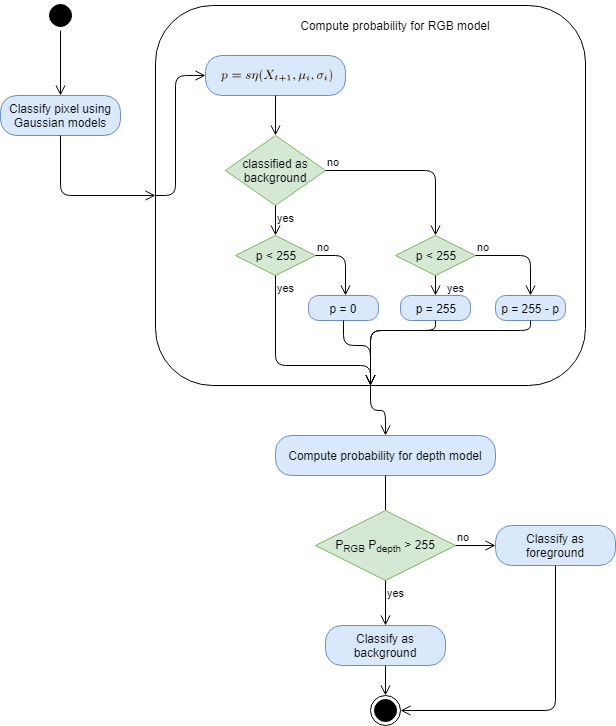
\includegraphics[scale=0.50]{img/gmm_alg.png}
		\caption{GMM -- computing probability and classification}
		\label{fig:gmm_alg}
	\end{center}
\end{figure}

\subsection{PBAS algorithm with RGBD sensor}
\label{subsec:pbas_rgbd}

The background model is composed of two parts. The first one is a buffer of $N$ last samples from the analyzed video sequence. Particular sample consists both RGB value and depth parameter. Let $x_i$ denote a particular pixel and $B(x_i)$ a buffer, it is described by equation (\ref{equ:pbas_model_1}).

%Modeł tła składa się z dwóch części. Pierwsza z nich zawiera $N$ ostatnich zapamiętanych próbek (wartości pikseli). Zapisywane są zarówno składowe RGB każdego piksela jak i parametr \textit{depth}. Definiujemy ten zbiór jako $B(x_i)$, gdzie $x_i$ to aktualnie przetwarzany piksel obrazu, całość została opisana równaniem (\ref{equ:pbas_model_1}).

	\begin{equation}
		B(x_i)= \left\{ B_1(x_i), B_2(x_i), \dotsc, B_N(x_i) \right\}
	\label{equ:pbas_model_1}	
	\end{equation}

The next component of background model is a sphere $S(v(x,y)$ of radius $R(x_i)$ centered at point $v(x,y)$. The radius value is updated with each new frame. Pixel is considered as foreground if at least $\#_{min}$ samples from background model belongs to the sphere. Let $F(x_i)$ denote the foreground mask (1 -- foreground pixel, 0 -- background), the match test is described by equation (\ref{equ:pbas_test}).

%Kolejnym elementem algorytmu jest okrąg $S(v(x,y)$ o środku w punkcie $v(x,y)$ i promieniu $R(x_i)$. Promień ten jest elementem modelu tła, aktualizowanym wraz z kolejnymi ramkami obrazu. Piksel jest uznawany za pierwszoplanowy jeżeli przynajmniej $\#_{min}$ próbek z modelu tła zawiera się wewnątrz takiego okręgu. Test dopasowania został opisany równaniem (\ref{equ:pbas_test}). Oznaczmy przez F maskę reprezentującą obiekty pierwszoplanowe (1 – piksel pierwszoplanowy, 0 – tło).

	\begin{equation}
	    F(x_i) = 
		\begin{dcases}
    		1, & \text{if } \sum_{k=0}^{N} \{ d(I(x_i), B_k(x_i)) < R(x_i) \} < \#_{min} \\
    		0, & \text{otherwise} 
		\end{dcases}
	\label{equ:pbas_test}	
	\end{equation}
\noindent Where $d$ is a distance function between a sample from background model and actual pixel.	
	
%\noindent Gdzie $d$ to funkcja odległości pomiędzy próbką z modelu tła, a aktualnym pikselem. 

Since each channel is processed separately, the distance function can be easily represented by equation (\ref{equ:pbas_dist}). The final decision is based on logical alternative of the result obtained for each channel. Let $F_R$, $F_G$, $F_B$, $F_D$ denote classification result for particular channels, final result is described by~(\ref{equ:pbas_final_mask}).

%Ponieważ każdy kanał analizowany jest osobno, funkcję odległości pomiędzy próbkami można zapisać bardzo prosto równaniem (\ref{equ:pbas_dist}), jest to po prostu moduł różnicy.

	\begin{equation}
		d(I(x_i),B_k(x_i)) = | I(x_i) - B_k(x_i) |
	\label{equ:pbas_dist}	
	\end{equation}

%Każdy kanał przetwarzany jest osobno z wykorzystaniem niezależnego modelu tła. Finalna maska jest alternatywą logiczną wyników z poszczególnych kanałów, oznaczając poszczególne maski jako $F_R$, $F_G$, $F_B$, $F_D$ ostateczną klasyfikację możemy zapisać równaniem~(\ref{equ:pbas_final_mask}).

    \begin{equation}
        F_{RGBD} = F_R \lor F_G \lor F_B \lor F_D
    \label{equ:pbas_final_mask}
    \end{equation}

In the next step the background model is updated. Proposed algorithm uses conservative update approach, it means that the model is updated only if classified pixel is a part of background, otherwise updater is skipped. In addition to conventional conservative approach, update decision is also randomized. The probability of performing an update is given as $p = 1/T(x_i)$, where $T(x_i)$ is independent for each pixel and updated with background model. The actual update procedure is based on replacing a randomly selected sample from the background model $B_k(x_i)$ with the current pixel value $I(x_i)$. Moreover, a random pixel from a $3x3$ local context is selected and a randomly selected sample from its model is replaced by pixel value. 


%Kolejnym krokiem po przeprowadzeniu testu dopasowania i klasyfikacji piksela jest aktualizacja modelu tła. Zastosowano konserwatywne podejście, czyli aktualizowane są tylko piksele sklasyfikowane jako tło. Decyzja o aktualizacji podejmowana jest losowo. Prawdopodobieństwo jej wykonania wynosi $p = 1/T(x_i)$, gdzie parametr $T(x_i)$ jest dynamicznie aktualizowany i niezależny dla każdego piksela. Sama aktualizacja, polega na nadpisaniu, losowo wybranej próbki $B_k(x_i)$ z modelu aktualną wartością piksela $I(x_i)$. Dodatkowo, wybierany jest losowy piksela z otoczenia $3x3$ i losowo wybrana próbka z modelu mu odpowiadającego, jest nadpisywana wartością tego piksela.


The update of $R(x_i)$ and $T(x_i)$ parameters is performed independently from the first part of background model. In this case the next component of the model has to be define -- the minimum distances between samples from the model and current pixel are defined as (\ref{equ:pbas_model_2}).

%Niezależnie od aktualizacji części modelu zawierającej zapamiętane próbki dokonywana jest zmiana parametrów $R(x_i)$ i $T(x_i)$. W tym celu konieczne jest zdefiniowanie kolejnego elementu modelu tła, który zawiera zbiór minimalnych odległości pomiędzy próbką z modelu a aktualną wartością piksela. Zbiór ten został opisany równaniem (\ref{equ:pbas_model_2}). 
 
	\begin{equation}
		D(x_i)= \left\{ D_1(x_i), D_2(x_i) \dotsc, D_N(x_i) \right\}
	\label{equ:pbas_model_2}	
	\end{equation}

Presented set of values -- $D(x_i)$ is updated together with the set of samples $B(x_i)$. If a pixel is updated the minimal distance is found with equation (\ref{equ:pbas_d_min}) and the value $D_k(x_i)$ is updated with~$d_{min}(x_i)$.  

%Przedstawiony zbiór $D(x_i)$ aktualizowany jest razem ze zbiorem próbek. Nadpisywany jest jedynie element o indeksie $k$ dla którego dystans pomiędzy próbką i aktualnym pikselem jest najmniejsza, zostało to przedstawione równaniem (\ref{equ:pbas_d_min}).
	
	\begin{equation}
		d_{min}(x_i) = min_k d(I(x_i), B_k(x_i))
	\label{equ:pbas_d_min}	
	\end{equation}

In $R(x_i)$ update procedure the background dynamics parameter is used, it is the mean value of $D(x_i)$, the whole procedure is described by equation (\ref{equ:pbas_r_update}). Additionally the decision threshold was limited by a lower bound $R_{low} = 18$.

%Do aktualizacji progu dopasowania, czyli parametru $R(x_i)$ konieczne jest wyznaczenie tzw. miary dynamiki tła, czyli inaczej wartości średniej ze zbioru $D(x_i)$. Finalny wzór na nową wartość progu przedstawia równanie (\ref{equ:pbas_r_update}). Warto dodać, że przyjęto także dolne ograniczenie wartości parametru, wynoszące $R_{low} = 18$.
    
    \begin{equation}
	    R(x_i) = 
		\begin{dcases}
    		R(x_i)(1-R_{inc/dec}), & \text{if } R(x_i) > \bar{d}_{min}(x_i)R_{sc} \\
    		R(x_i)(1+R_{inc/dec}) & \text{otherwise} 
		\end{dcases}
	\label{equ:pbas_r_update}	
	\end{equation}

Where:
\begin{itemize}
	\item[$R_{inc/dec}$] -- constant updater rate ($0.05$ by default)
	\item[$\bar{d}_{min}(x_i)$] -- the mean value of $D(x_i)$
	\item[$R_{sc}$] -- scaling factor ($5$ by default)
\end{itemize}

%Gdzie:
%\begin{itemize}
%	\item[$R_{inc/dec}$] -- stały współczynnik aktualizacji (domyślnie $0.05$)
%	\item[$\bar{d}_{min}(x_i)$] -- wartość średnia zbioru $D(x_i)$
%	\item[$R_{sc}$] -- współczynnik skalowania (domyślnie $5$)
%\end{itemize}

The final step is update of learning rate parameter -- $T(x_i)$. The new value depends on classification result and it is described as (\ref{equ:pbas_t_update}). Additionally
the learning rate is limited by a lower and upper bound. These constraints are $T_{low}=2$ and $T_{up}=200$ respectively.

%Ostatni etap to aktualizacja parametru opisującego prawdopodobieństwo dokonania aktualizacji, czyli $T(x_i)$. Nowa wartość zależy od wyniku klasyfikacji piksela i została opisana równaniem (\ref{equ:pbas_t_update}). Przyjęto założenie, że parametr ten posiada także ograniczenie dolne jak i górne wynoszące odpowiednio $T_{low}=2$ i $T_{up}=200$. 

    \begin{equation}
	    T(x_i) = 
		\begin{dcases}
    		T(x_i) + \frac{T_{inc}}{\bar{d}_{min}(x_i)}, & \text{if } F(x_i)=1 \\
    		T(x_i) - \frac{T_{dec}}{\bar{d}_{min}(x_i)} & \text{otherwise} 
		\end{dcases}
	\label{equ:pbas_t_update}	
	\end{equation}

\section{Hardware implementation}
\label{sec:hw_implementation}

\subsection{Hardware used}
\label{subsec:hw_used}

For image acquisition Intel RealSense Depth Cameras D415 and D435 have been used. They provide the Full HD resolution ($1920x1080$) for RGB image and HD resolution ($1280x720$) for depth map. Those sensors are able to distinguish objects at a distance of 20 centimeters to 10 meters from camera~lens.

%Do akwizycji obrazu użyto czujników RGB--D firmy Intel: REAL SENSE Depth Camera D415 oraz REAL SENSE Depth Camera D435. Zapewniają
%one obraz w maksymalnej rozdzielczości FULL HD (1920 x 1080 pikseli) oraz mapę głębi w rozdzielczości HD (1280 x 720 pikseli). Sam czujnik umożliwia rozróżnianie obiektów w odległości od 20 centymetrów do 10 metrów od obiektywu.

%Presented algorithms were implemented on three different platform. The first one is embedded GPU, NIVIDIA Jetson TX2, it consists of ARM based CPU and GPU. The second platform is notebook with Intel Core i7--7700 processor and mobile version of Geforce GTX 1050. 

For hardware implementation 3 different platforms were used. The first one is Nvidia Jetson TX2 -- embedded GPU platform, equipped with 64-bits ARM Cortex A57 CPU and NVIDIA Maxwell GPU with 256 CUDA cores. The second platform is laptop with Intel Core i7--7700HQ (4 cores/8 threads @ 2.8 GHz) and NVIDIA Geforce GTX 1050 GPU based on Pascal architecture. Last but not least is PC consisting of Intel Core i7--9700k (8 cores @ 4.5 GHz) and NVIDIA RTX 2070 (Touring architecture).

%Algorytm zaimplementowano na 3 różnych platformach sprzętowych. Pierwszą jest układ embedded GPU NVIDIA Jetson TX2 wyposażony w procesor ARM i układ GPU. Druga platforma to laptop wyposażony w procesor intel core i7-7700 i kartę graficzną Geforce GTX 1050m. Najwydajniejsza z testowanych platforma to komputer PC z intel Core i7-9700k i NVIDIA Geforce RTX 2070.

Most calculations are made with the use of GPU, for this purpose the CUDA (\textit{Copute Unififed Device Architecture}) platform was used. It is developed by NVIDIA and can be used only with GPUs based on their architecture. The CUDA itself is parallel computing platform with API which allows to use NVIDIA graphics processing unit for general purpose processing. Thanks to this approach we can integrate our implementation with different computing platforms like laptops, PCs or embedded GPUs without much effort. The only requirement is to use NVIDIA GPU. 

%\textbf{TODO: dokonczyc wstep}

%Do implementacji sprzętowej wykorzystano opracowaną przez Nvidia architekturę CUDA ( Compute Unified Device Architecture). Dzięki temu implementacja może zostać uruchomiona na dowolnym układzie embedded GPU lub komputerze osobistym, które są wyposażone w procesor graficzny Nvidia. 

\subsection{Architektura}
\label{subsec:architecture}

Distribution of tasks between CPU and GPU is one of the key element in implementation of such a hardware accelerated system. The host (CPU) is responsible for image acquisition and copying date to shared GPU memory (DRAM). Moreover, the memory allocation is also provided by host, it is required to reserve memory for background model. Communication between host and GPU is done over PCI bus. Basic architecture scheme is shown in the figure \ref{fig:cpu_host}.    

%Jednym z najistotniejszych elementów jest podział zadań pomiędzy hostem i układem GPU oraz wykorzystanie pamięci współdzielonej. Host odpowiada za akwizycję obrazu i następnie skopiowanie go do pamięci współdzielonej z GPU. Oprócz tego po stronie hosta wykonywana jest również alokacja pamięci wykorzystywanej przez GPU, w związku z tym konieczne jest także zarezerwowanie pamięci dla modelu tła. Komunikacja odbywa się po szynie PCI, zostało to pokazane na rysunku \ref{fig:cpu_host}. 


\begin{figure}[!t]
	\begin{center}
		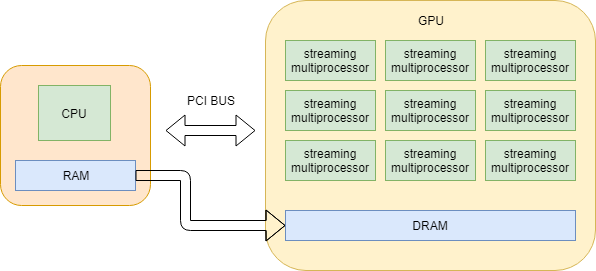
\includegraphics[scale=0.50]{img/cpu_host.png}
		\caption{Communication between host (CPU) and GPU}
		\label{fig:cpu_host}
	\end{center}
\end{figure}

Every job related with foreground segmentation is implemented in GPU, while CPU is responsible for simple pre and post processing tasks. It allows to process each pixel parallel, independently, using separate thread. The output of the system is binary mask containing foreground objects. This mask has to be copied from GPU DRAM memory to CPU RAM and then forwarded to external display. The entire callstack and process of exchanging data between host and cpu is shown in the figure \ref{fig:gpu_alg}.


%Właściwy algorytm został w całości zaimplementowany na procesorze graficznym, gdzie dla każdego przetwarzanego piksela tworzony jest osobny wątek. Wyjściem algorytmu jest maska binarna przedstawiająca obiekty pierwszoplanowe, jest umieszczona w pamięci współdzielonej i następnie odczytana przez hosta i przekazana na wyjście. Proces wymiany informacji pomiędzy hostem i gpu został pokazany na rys. \ref{fig:gpu_alg}.

Implementacja po stronie hosta została napisana w języku \textit{C++}. Do akwizycji obrazu wykorzystano udostępnione przez firmę \textit{Intel} SDK do obsługi sensorów RGB--D. Umożliwia ona odczyt zarówno obrazu RGB z kamery  jak i składowej głębi w czasie rzeczywistym. Obraz głębi jest przesyłany z czujnika w formacie zmiennoprzecinkowym, zatem przed przesłaniem go do GPU konieczna jest konwersja do formatu 8 bitów na pixel (większa wartość oznacza, że obiekt jest dalej od kamery). Ostatecznie każdy piksel obrazu jest zapisany na 32 bitach, po 8 bitów na każdą składową RGB oraz odległość od czujnika. 

\begin{figure}[!t]
	\begin{center}
		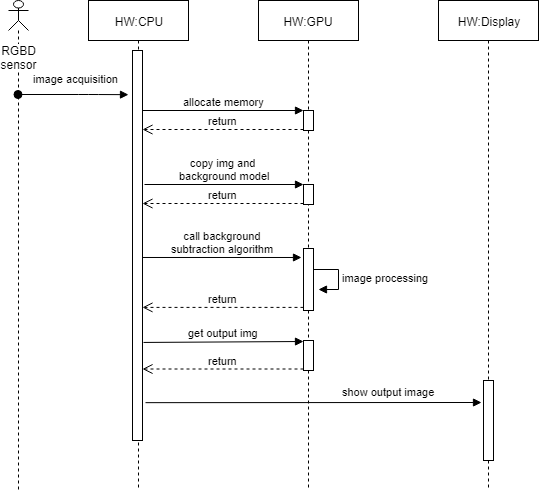
\includegraphics[scale=0.50]{img/gpu_bs_alg.png}
		\caption{}
		\label{fig:gpu_alg}
	\end{center}
\end{figure}

%\subsection{GMM implementation}
%\label{subsec:gmm_implementation}


%\subsection{PBAS implementation}
%\label{subsec:pbas_implementation}


\subsection{Performance}
\label{subsec:performance}

Wydajność na poszczególnych platformach testowych została zmierzona dla różnych rozdzielczości: 480p/480p, 720p/480p, 720p/720p, 1080p/720p, gdzie poszczególne wartości przedstawiają odpowiednio rozdzielczości obrazu i mapy głębi. Szczegółowe wyniki dla poszczególnych układów GPU zostały przedstawione w tabeli \ref{tab:performance_res}.

%\textbf{TODO: tabelka z pomiarami}

\begin{table}[t!]
\caption{Performance}
\centering
\begin{tabular}{|c|c|c|c|c|c|}
\hline
&     480p/480p  & 720p/480p & 720p/720p & 1080p/720p \\ \hline
Nvidia Jetson TX2  & XXfps & XXfps & XXfps & XXfps  \\ \hline
i7 7700hq + GTX 1050   & XXfps & XXfps & XXfps & XXfps     \\ \hline
i7 9700k + RTX 2070 & XXfps & XXfps &  XXfps & XXfps    \\ \hline
Nvidia Jetson Xavier  & XXfps    & XXfps    & XXfps & XXfps     \\ \hline
\end{tabular}
\label{tab:performance_res}
\end{table}

\textbf{TODO:}\\
-> zrzut ekranu\\
%->opis komunikacji pomiędzy hostem i GPU + rysunek,\\ 
%->standardowy algorytm segmetnacji obiektów (model tła, znajduje się w pamięci współdzielonej), \\
%->opisać co zrobione w OpenCV, a co w CUDA, problem podziału zadań 
%biblioteka intela,\\
%->wykorzystane urządzenia - specyfikacja,\\
%->przekonwertowanie do tej samej rozdzielczości,\\
%->opis zastosowanych modułów,\\
%->w przypadku PBASa z indeksacją można dużo zrobić, np własna indeksacja w CUDA (-to moze w conclusion),\\
%->implementation result,\\
->wydajność--wnioski


\section{Evaluation}
\label{sec:evaluation}

W celu przetestowania zaimplementowanych algorytmów przygotowano krótkie sekwencje testowe nagrane kamerą RGB--D. Do każdego nagrania został przygotowany \textit{ground truth}, czyli ręcznie anotowana maska obiektów. Wartość 255 oznacza, że dany piksel jest obiektem pierwszoplanowym, natomiast 0 oznacza tło. Wyjście w 100\% poprawnego algorytmu powinno pokrywać się z tą maską. 

Do ewaluacji użyto metodologii znanej między innymi z portalu \textit{Change Detection} \cite{}. Porównują ramki wyjściowe testowanego algorytmu z odpowiadającymi im ramkami modelu wzorcowego, można wyznaczyć następujące współczynniki:

\begin{enumerate}
\item[TP] – liczba pikseli poprawnie zakwalifikowanych jako pierwszy plan (ang. true positive)
\item[TN] – liczba pikseli poprawnie zakwalifikowanych jako tło (ang. true negative)
\item[FN] – liczba pikseli błędnie zakwalifikowanych jako tło (ang. false negative)
\item[FP] – liczba pikseli błędnie zakwalifikowanych jako pierwszy plan (ang. false positive)
\end{enumerate}

\noindent Na podstawie wyznaczonych współczynników oblicza się 4 wskaźniki jakości określających dokładność metody:

\begin{enumerate}

\item Precision (Pr): $TP/(TP + FP)$
\item Specificity (Spec) : $TN/(TN + FP)$
\item Recall (Re) : $TP/(TP + FN)$
\item Percentage of Wrong Classifications (PWC) : $100(FN + FP)/(TP + FN + FP + TN)$

\end{enumerate}

Podczas testów użyto własnoręcznie nagranych krótkich sekwencji video, nagranych za pomocą czujnika Intel RealSense. Wzorowa maska binarna została opracowana manualnie, z wykorzystaniem algorytmów segmentacji znajdujących się w bibliotece OpenCV. Uzyskane wyniki porównano z oryginalnymi implementacjami algorytmów GMM \cite{} i PBAS \cite{}, szczegółowe wyniki zamieszczono w tabeli \ref{tab:evaluation_res}.


\begin{table}[t!]
\caption{Evaluation}
\centering
\begin{tabular}{|c|c|c|c|c|c|}
\hline
&     GMM RGB--D  & PBAS RGB--D & GMM \cite{} & PBAS \cite{} \\ \hline
Re  & XX & XX & XX & XX  \\ \hline
Spec   & XX & XX & XX & XX     \\ \hline
FPR & XX & XX &  XX & XX    \\ \hline
FNR  & XX    & XX    & XX & XX     \\ \hline
PWC  & XX    & XX    & XX & XX     \\ \hline
Pr  & XX    & XX    & XX & XX     \\ \hline
F1  & XX    & XX    & XX & XX     \\ \hline
\end{tabular}
\label{tab:evaluation_res}
\end{table}


\textbf{TODO:}\\
% ->ewaluacja algorytmów, \\
 %->nagrane sekwencje testowe, \\
 %->opracowanie groundtrue, \\
 %->zastosowane współczynniki, \\
 %->porównanie z oryginalnymi implementacjami (wyniki z publikacji artykułach ???)
 ->wnioski z wyników



\section{Conclusion}
\textbf{TODO:}\\
->w przypadku PBASa z indeksacją można dużo zrobić, np własna indeksacja w CUDA\\
->implementacja FPGA w przyszlosci ???\\
->wykorzystanie RGBD == większa dokładność (plus kilka procent)\\
->nikt tego wcześniej nie robił\\
->dodać bib\\
->zmienić szablon\\

%\bibliographystyle{plain}
%\bibliography{cars}



\end{document}
